\documentclass{article}
\usepackage{graphicx} % Required for inserting images
\usepackage[italian]{babel}
\usepackage{amsmath}
\usepackage[hidelinks]{hyperref}
\usepackage{amssymb}
\usepackage{changepage}
\usepackage{float}
\usepackage{algorithm}
\usepackage{algpseudocode}

\title{Metodi matematici per l'informatica}
\author{Leonardo Ganzaroli}
\date{}

\begin{document}

\maketitle

\addcontentsline{toc}{section}{\protect\numberline{}Introduzione}

\tableofcontents

\newpage

\hypersetup{allcolors=black}

\section*{Introduzione}

Questi appunti sono derivanti principalmente dalle dispense del corso di \textit{Metodi matematici per l'informatica} che ho svolto durante la laurea Triennale di informatica all'università "La Sapienza".

\newpage

\section{Richiami sugli insiemi}

\begin{enumerate}
    \item Un insieme è una collezione di elementi
    \item Un insieme può essere definito in 2 modi:
    \begin{itemize}
    
        \item Per elencazione

            \qquad $X=\{1,3,x,@\}$

        \item Per proprietà caratteristica

            \qquad $Y=\{x\ |\ x \text{ è una casa}\}$
        
    \end{itemize}

    \item La cardinalità di un insieme è il numero di elementi che esso contiene

    \item Se un insieme ha cardinalità finita allora è detto "finito"

    \item L'insieme vuoto si indica con $\emptyset$

    \item L'insieme potenza di un certo insieme è l'insieme dei suoi sottoinsiemi

    \item Il prodotto cartesiano di 2 insiemi è l'insieme delle coppie ordinate $(x,y)$ con $x$ appartenente al primo insieme e $y$ al secondo

\vspace{10pt}
    
\end{enumerate}

Le operazioni tra insiemi (dati A e B):
\vspace{5pt}
\begin{itemize}
    \item \textbf{Unione} ($A\cup B$) = L'insieme contenente tutti gli elementi di A e di B
    \item \textbf{Intersezione} ($A\cap B$)= L'insieme contenente gli elementi comuni di A e di B

    \item \textbf{Differenza} ($A\setminus B$) = L'insieme contenente gli elementi di A che non appartengono a B
    
\end{itemize}

\vspace{10pt}

Le relazioni tra insiemi (dati A e B):
\vspace{5pt}
\begin{itemize}

    \item \textbf{Inclusione} ($A\subseteq B$) =  A è un sottoinsieme di B, ossia B contiene tutti gli elementi di A

    \item \textbf{Inclusione propria} ($A\subset B)$ = Come sopra ma B contiene elementi aggiuntivi non presenti in A

    \item 2 insiemi si dicono \textbf{Coincidenti} ($A\subseteq B\ \text{e} \ B\subseteq A$ ) se sono lo stesso insieme, ossia hanno gli stessi elementi

    \item 2 insiemi si dicono \textbf{Disgiunti} ($A\cap B = \emptyset$) se non hanno nessun elemento in comune
    
\end{itemize}

\newpage

\section{Combinatoria}

Per combinatoria si intende lo studio del contare gli insiemi finiti, risponde a domande del tipo:
\begin{itemize}
    \item  Quanti numeri primi esistono tra 1 e 1 milione?
    \item  Quante targhe è possibile formare nel sistema attualmente in uso in Italia?
    \item  Quanti sono gli esiti del lancio di 2 dadi a 6 facce?
    \item \ldots
\end{itemize}

\subsection{Principio moltiplicativo}

\textbf{Definizione} Se scelgo un primo oggetto tra $a$ disponibili, un secondo tra $b$, un terzo tra $c$, \ldots, un ultimo tra $z$ allora ho: $$a\times b \times c \times \ldots \times z\  \text{  possibili scelte}$$

\noindent\rule{\textwidth}{0.5pt}

\noindent Esempio:\newline

\noindent A una gara di corsa partecipano 8 atleti. Quanti sono i possibili ordini di arrivo, assumendo che
tutti arrivino al traguardo e che non vi siano arrivi simultanei?\newline

\noindent Applicando il principio ottengo $8*7*6*5*4*3*2*1 = 40320$

\noindent\rule{\textwidth}{0.5pt}

\subsection{Principio additivo}

\textbf{Definizione} Per contare gli oggetti che soddisfano un certo vincolo posso:
\begin{enumerate}
    \item Trovare delle categorie non sovrapposte che descrivano la totalità degli oggetti con quel vincolo
    \item Dividere gli oggetti nelle categorie
    \item Sommare il numero di oggetti in ciascuna categoria
\end{enumerate}

\noindent Si può riformulare anche dal punto di vista insiemistico.\newline

\noindent\textbf{Definizione} Sia A un insieme e $T_1,T_2,\ldots,T_k$ una partizione di A, si ha: $$\#A = \#T_1+\#T_2+\ldots+\#T_k$$

\newpage

\noindent\rule{\textwidth}{0.5pt}

\noindent Esempio:\newline

\noindent In una gara di 8 atleti di cui 2 italiani, 3 francesi e 3 spagnoli, quanti sono gli ordini di arrivo
in cui i primi tre atleti hanno nazionalità diverse?\newline

Trovo i possibili casi esclusivi:
\begin{enumerate}
    \item \textbf{IFS} = \{ordini di arrivo con un Italiano primo, un Francese secondo e uno Spagnolo terzo\}
    \item \textbf{ISF} = \{ordini di arrivo con un Italiano primo, uno Spagnolo secondo e un Francese terzo\}
    \item \textbf{FIS} = \{ordini di arrivo con un Francese primo, un Italiano secondo e uno Spagnolo terzo\}
    \item \textbf{FSI} = \ldots
    \item \textbf{SIF} = \ldots
    \item \textbf{SFI} = \ldots
\end{enumerate}

Posso adesso calcolare il risultato sommando le cardinalità degli insiemi.

\noindent\rule{\textwidth}{0.5pt}

\subsection{Figure}

Avendo visto i 2 principi base possiamo adesso passare alle \textit{figure} ricorrenti della combinatoria.

\subsubsection{Disposizioni con ripetizione}

\textbf{Definizione} Una disposizione con ripetizione di ordine $k$ di $n$ oggetti è una sequenza ordinata di $k$ oggetti scelti tra gli $n$ totali.

$$D_{n,k}'=n\times n \times n \times \ldots = n^k$$

\vspace{4pt}

\noindent\rule{\textwidth}{0.5pt}

\noindent Esempio: Le possibili parole di lunghezza 5 dell'insieme \{a,b,c\} sono $D_{3,5}'=3^5$

\noindent\rule{\textwidth}{0.5pt}

\subsubsection{Disposizioni semplici}

\textbf{Definizione} Dato $1\leq k \leq n$. Una disposizione semplice di ordine $k$ di $n$ oggetti è una sequenza ordinata di $k$ oggetti distinti scelti tra gli $n$ totali.

$$D_{n,k}=n\times (n-1) \times (n-2) \times \ldots \times (n-(k-1)) = \frac{n!}{(n-k)!}$$

\vspace{2pt}

\noindent\rule{\textwidth}{0.5pt}

\noindent Esempio:\newline  

\noindent Se ad un torneo partecipano 8 squadre scelte tra 15 e l’ordine di partenza è a sorte,
quanti sono i possibili schieramenti di partenza?\newline

\noindent Soluzione = $D_{15,8} = \frac{15!}{(15-8)!}= \frac{15!}{7!}$

\noindent\rule{\textwidth}{0.5pt}

\subsubsection{Permutazioni}

Se una disposizione semplice ha $n=k$ si parla di permutazione: $P_n=D_{n,n}=n!$

\subsubsection{Anagrammi}

Gli anagrammi sono un caso particolare di disposizione in cui ci sono dei "gruppi" di lettere ripetute.

$$\#A = \frac{n!}{n_1!n_2!n_3!\ldots}$$

\noindent\rule{\textwidth}{0.5pt}

\noindent Esempio: Gli anagrammi della parola MISSISSIPPI sono $\frac{11!}{4!4!2!}$

\noindent\rule{\textwidth}{0.5pt}

\subsubsection{Combinazioni semplici}

\textbf{Definizione} Le combinazioni semplici di ordine $k$ su $n$ sono i sottoinsiemi di
$k$ elementi scelti in un insieme di $n$ elementi.

$$C_{n,k}=\frac{D_{n,k}}{k!}=\frac{n!}{(n-k)!*k!}=\binom{n}{k}$$

\noindent\rule{\textwidth}{0.5pt}

\noindent Esempio:\newline

\noindent Dato $A=\{a,b,c,d\}$ calcolare il numero di sottoinsiemi di 3 elementi.\newline

\noindent Soluzione = $\binom{4}{3}=4$\newline\rule{\textwidth}{0.5pt}

\vspace{5pt}

\noindent Un caso specifico è quello in cui ci si trova con la formula $\binom{n}{m}\times m$, infatti essa risulta equivalente alla formula $n\times \binom{n-1}{m-1}$.\newline

\noindent Data la sua definizione si può trovare la seguente correlazione tra l'insieme potenza e le possibili combinazioni dello stesso insieme:

$$\text{Dato A insieme e } n=\#A \text{ si ha } \sum_{x=0}^n \binom{n}{x} = \#P(A)$$

\subsubsection{Combinazioni con ripetizioni}

\textbf{Definizione} Le combinazioni con ripetizione di ordine $k$ di $n$ oggetti sono un raggruppamento di
$k$ oggetti scelti tra $n$ elementi con possibili ripetizioni.

$$C_{n,k}'=\binom{n+k-1}{n-1}$$

\subsubsection{Principio di inclusione-esclusione}

Si possono presentare dei casi in cui sia necessario usare il principio additivo ma non è possibile creare dei tipi mutualmente esclusivi, in questo caso si andrebbero a contare degli elementi più di una volta portando ad un risultato sbagliato.\newline

\noindent Per ovviare al problema vanno rimossi gli elementi comuni per non contarli più volte:

$$\#(A\cup B) = \#A+\#B-\#(A\cap B)$$\newline

\noindent Nel caso siano 3 insiemi va reinserita la parte comune a tutti e 3, altrimenti resterà fuori dalla somma:

\vspace{-8pt}

$$\#(A \cup B \cup C) = \#A + \#B + \#C - \#(A \cap B) - \#(A \cap C) - \#(B \cap C) + \#(A \cap B \cap C)$$\newline

\vspace{-5pt}

\noindent \textit{Più in generale vanno aggiunte le operazioni con numero di elementi dispari e tolte quelle con numero di elementi pari.}

\section{Relazioni}

\textbf{Definizione}  Siano A e B due insiemi. Una relazione R tra A e B è un sottoinsieme del
prodotto cartesiano $A\times B$.\newline

\noindent Per indicare che 2 elementi sono in relazione tra loro si può scrivere $R(a,b)$ oppure $aRb$.

\subsection{Rappresentazione}

Per rappresentare graficamente una relazione ho 2 alternative:
\begin{enumerate}
    \item \textbf{Matrice}

    Si utilizza una matrice in cui il valore di una singola cella è descritto da:
    
\[
m_{ij} =
\begin{cases}
1 & \text{se } (a_i, b_j) \in R \\
0 & \text{se } (a_i, b_j) \notin R
\end{cases}
\]

\noindent\rule{\textwidth}{0.5pt}

Esempio:\newline

 Siano $A = \{1, 2, 3, 4\} \text{ e } R = \{(1, 2),(2, 4),(3, 2),(4, 2),(4, 4)\}$.

 $$ M_R = \begin{pmatrix}

    0 & 1 & 0 & 0\\
    0 & 0 & 0 & 1\\
    0 & 1 & 0 & 0\\
    0 & 1 & 0 & 1
     
 \end{pmatrix}$$

\noindent\rule{\textwidth}{0.5pt}

\item \textbf{Grafo diretto}

    A SX gli elementi del primo insieme, a DX quelli del secondo,
    disegno una freccia da SX a DX solo se quella coppia è nella relazione.

\noindent\rule{\textwidth}{0.5pt}

Esempio:\newline

 Siano $ A = \{a,b,c,d,e\}, \ B = \{1,2,3,4,5\} \text{ e } R=\{(a, 2),(b, 4),(c, 2),(e, 1),(e, 4)\}$.

    \begin{figure}[ht]
        \centering
        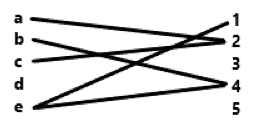
\includegraphics[width=0.4\linewidth]{grafo.png}
        \caption{Grafo diretto}
        \label{fig:grafo}
    \end{figure}

\noindent\rule{\textwidth}{0.5pt}
    
\end{enumerate}

\subsection{Inversa}

\textbf{Definizione} Data una relazione $R\subseteq A\times B$. Si definisce $R^{-1}$ (inversa di R) il sottoinsieme di $B\times A$ tale che:

$$R^{-1} = \{(b,a)\ |\ (a,b)\in R\}$$

\subsection{Composizione}

\textbf{Definizione} Date $R\subseteq A \times B$ e $S\subseteq B\times C$. Si definisce composizione di $R$ ed $S$ ($S\circ R$) la relazione tra $A$ e $C$ in cui:
$$(a,c) \in (S\circ R) \text{ con } a\in A,\ c\in C \iff \exists b\in B\ |\ aRb \text{ e } bSc$$

\subsection{Rel. transitive}

\textbf{Definizione} Una relazione $R\subseteq A\times A$ è transitiva se: 
$$\forall \  a,b,c \in A \ \ aRb \text{ e } bRc\ \Rightarrow\  aRc $$

\subsubsection{Chiusura transitiva}

\textbf{Definizione} La chiusura transitiva di una relazione $R$ è la più piccola relazione transitiva che estende $R$ (definita $R^T$) tale che:
\begin{enumerate}
    \item $R\subseteq R^T$
    \item $R^T$ è transitiva
    \item Se $S$ estende $R$ ed è transitiva allora $R^T\subseteq S$\newline
\end{enumerate}

\noindent Estendendo il discorso si può definire una relazione di raggiungibilità definita come:

$$R^C=\{(a,b)\in A\times A \ | \ \exists \text{ un cammino di lunghezza $\geq 1$ da $a$ verso $b$} \}$$

\subsection{Rel. di equivalenza}

\textbf{Definizione} Una relazione $R\subseteq A\times A$ è detta di equivalenza se gode di queste proprietà:
\begin{itemize}
    \item \textbf{Riflessività} $\forall\ a\in A\ \  aRa$
    \item \textbf{Simmetria} $\forall\ a,b\in A\ \ aRb\ \Rightarrow\ bRa$
    \item \textbf{Transitività} (Vista prima)\newline
\end{itemize}

\noindent\textbf{Definizione} La classe di equivalenza di un elemento di $A$ è definita come:

$$[a]_R=\{b\in A\ |\ aRb\}$$

\noindent Inoltre:
\begin{itemize}
    \item $\forall\ a\in A\ \ [a]_r\neq \emptyset$
    \item $\forall\ a,b\in A \ \ [a]_r\ \cap\ [b]_r = \emptyset\ \text{ oppure } [a]_r=[b]_r $
\end{itemize}

\noindent Questo dimostra che ogni relazione di equivalenza su un insieme crea una partizione di quell'insieme.\newline

\newpage

\noindent Posso formulare la partizione come:

$$\{C_i\ |\ i\in I\} \text{ con } I= \text{insieme di indici qualunque, } C_i\neq\emptyset \text{ e } C_i\subseteq A$$

\vspace{2pt}

\noindent Valgono:
\begin{enumerate}
    \item $\forall\ a\in A \ \ \exists i\in I\ |\ a\in C_i$
    \item $\forall \ i,j\in I\ \ i\neq j\ \Rightarrow\ C_i\ \cap\ C_j = \emptyset $
\end{enumerate}

\subsection{Rel. d'ordine}

\textbf{Definizione} Una relazione $R\subseteq A\times A$ è detta di ordine parziale se gode di queste proprietà:
\begin{itemize}
    \item \textbf{Riflessività} (Vista prima)
    \item \textbf{Antisimmetria} $\forall\ a,b\in A\ \ aRb  \text{ e } bRa\ \Rightarrow\ a=b$
    \item \textbf{Transitività} (Vista prima)
    \item \textbf{Totalità} (Se vale questa proprietà la relazione è d'ordine totale) 
    
    $\forall\ a,b\in A\ \ a\leq b \text{ oppure } b\leq a$\newline
\end{itemize}

\noindent In caso di ordini parziali finiti posso rappresentare graficamente la relazione con il diagramma di Hasse.

\noindent\rule{\textwidth}{0.5pt}

\noindent Esempio:\newline

\noindent Diagramma della relazione d'ordine "$\leq$" nell'insieme dei divisori del 60.

    \begin{figure}[ht]
        \centering
        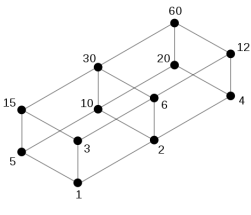
\includegraphics[width=0.5\linewidth]{hasse.png}
        \caption{Diagramma di Hasse}
        \label{fig:hasse}
    \end{figure}

\noindent\rule{\textwidth}{0.5pt}\newline

\newpage

\noindent Partendo da una relazione parziale $R$ è possibile trovare una relazione totale $R^*$ che va ad estenderla, basta che siano presenti nella nuova relazione:
\begin{itemize}
    \item Le coppie $(a,b)$ incomparabili di $R$
    \item Tutte le coppie $(x,y)$ tali che $xRa$ o $bRy$
\end{itemize}

\section{Funzioni}

\textbf{Definizione} Una funzione è una relazione tra due insiemi che associa ad ogni elemento del dominio (il primo insieme) un solo elemento del codominio (il secondo insieme):

$$\textit{f}: A \rightarrow B$$\newline

\noindent Dato un elemento $x$ del dominio che la funzione associa all'elemento $y$ del codominio si dice che:
\begin{itemize}
    \item $y$ è l'immagine di $x$ via \textit{f}
    \item $x$ è la pre-immagine di $y$ via \textit{f}
\end{itemize}

\subsection{Tipi}

\begin{itemize}
    \item \textbf{Iniettiva}

    Una funzione è iniettiva se $\forall \ x,y\in \text{Dominio}\ \ \textit{f}(x) = \textit{f}(y) \ \Rightarrow\ x=y$

    \item \textbf{Suriettiva}

    Una funzione è suriettiva se $\forall \ y\in \text{Codominio}\ \ \exists x\in \text{Dominio}\ |\ \textit{f}(x) = y$

    \item \textbf{Biunivoca}

    Una funzione è biunivoca se è sia iniettiva che suriettiva
    
\end{itemize}

\subsection{Composizione}

\textbf{Definizione} Siano $f:X\rightarrow Y$ e $g:Y\rightarrow Z$. La funzione composta di $f$ e $g$ $(g\circ f)$ è definita come:

$$h:X\rightarrow Z,\ h(x)=g(f(x))$$\newline

\noindent\textbf{N.B. Questa operazione non è commutativa}.

\subsection{Identità}

\textbf{Definizione} La funzione identità è quella che associa ad ogni elemento l'elemento stesso (ovviamente dominio e codominio sono uguali).\newline

\noindent Si indica con $\text{id}_{NOME\_INSIEME}$.

\subsection{Inversa}

\textbf{Definizione} Sia $\textit{f} :X\rightarrow Y$ una funzione. Un'altra funzione $\textit{g}:Y\rightarrow X$ si dice inversa di \textit{f} se:
\begin{enumerate}
    \item $(\textit{g}\circ \textit{f})$ è l'identità su $X$
    \item $(\textit{f}\circ \textit{g})$ è l'identità su $Y$\newline
\end{enumerate}

\noindent La funzione inversa di $f$ si denota con $\textit{f}^{-1}$.\newline

\noindent Una funzione è invertibile solo se è biunivoca.

\section{Cardinalità degli insiemi}

Si possono adesso legare le cardinalità degli insiemi alle funzioni tra di essi, dati $A$ e $B$:
\begin{itemize}
    \item Se esiste una funzione iniettiva tra i due allora $\#A\leq \#B$
    \item Se esiste una funzione iniettiva tra i due allora $\#A\geq \#B$
    \item Se esiste una funzione biunivoca tra i due allora $\#A= \#B$
\end{itemize}

\subsection{Insiemi numerabili}

Viene definito numerabile un insieme finito oppure per cui esiste una funzione biunivoca con $\mathbb{N}$ (in questo caso si dice infinito numerabile).

\subsection{Insiemi non numerabili}

Rientrano in questa categoria tutti gli insiemi per cui non esiste una funzione biunivoca con $\mathbb{N}$.

\newpage

\section{Induzione}

Il principio d'induzione serve a dimostrare che se una proprietà vale per il numero 0/1 allora vale per ogni numero $n$.\newline

\noindent Il procedimento è composto da 2 passi:
\begin{enumerate}
    \item \textbf{Base} 
    
    Verificare che la proprietà valga per 0/1
    \item \textbf{Passo induttivo} 
    
    Assumendo che la proprietà sia valida per un numero $n$ dimostrare che è valida anche per $n+1$
\end{enumerate}

\noindent\rule{\textwidth}{0.5pt}

\noindent Esempio:\newline

\noindent Dimostrare che $\sum_{x=0}^nx=\frac{n(n+1)}{2}$.
\begin{enumerate}
    \item \textbf{Base} 
    
    Se $n=1$ risulta $\frac{1(1+1)}{2}=1$, quindi è vero
    \item \textbf{Passo induttivo}

    Dando per buona la formula per $n$ devo dimostrare che $1+2+\ldots+n+n+1=\frac{(n+1)(n+2)}{2}$.\newline

    Si può notare che la somma fino ad $n$ si può trasformare in $\frac{n(n+1)}{2}$, che sappiamo essere corretta.\newline

    Si ottiene quindi $\frac{n(n+1)}{2}+n+1$ che con qualche passaggio diventa $\frac{(n+1)(n+2)}{2}$.\newline

    Questa proprietà risulta quindi vera.
    
\end{enumerate}

\noindent\rule{\textwidth}{0.5pt}\newline

\noindent Si puo anche generalizzare  e dimostrare che una proprietà valga dal numero $k$ in poi:
\begin{enumerate}
    \item \textbf{Base} 
    
    Verificare che la proprietà valga per k
    \item \textbf{Passo induttivo} 
    
    Assumendo che la proprietà sia valida per un numero $n\geq k$ dimostrare che è valida anche per $n+1$
\end{enumerate}

\subsection{Induzione forte}

Una variante del principio d'induzione in cui si lavora con gli insiemi, se un insieme $X$ ha queste caratteristiche:
\begin{enumerate}
    \item Contiene 1/0
    \item Se contiene tutti i numeri minori di un certo $n\geq 1$ allora contiene anche $n+1$\newline
\end{enumerate}

\noindent Si può concludere che $X=\mathbb{N}$

\subsection{Principio del minimo intero}

\textbf{Definizione} Ogni sottoinsieme non vuoto dei numeri naturali ha un minimo.\newline

\noindent Questo principio è essenzialmente una formulazione alternativa di quello d'induzione.
 
\section{Logica proposizionale}

La logica proposizionale si occupa delle proprietà dei costrutti logici usati nei linguaggi formali, tra questi ci sono quello naturale e quelli usati nelle scienze e nella matematica.\newline

\noindent Nel nostro caso i costrutti logici sono:
\begin{itemize}
    \item Il \textbf{non}
    \item L'\textbf{oppure}
    \item L'\textbf{e}
    \item Il \textbf{se \ldots allora}
    \item Il \textbf{se e solo se}
\end{itemize}

\subsection{Alfabeto e proposizioni}

L'alfabeto della logica è formato da:
\begin{itemize}
    \item Un insieme numerabile di simboli di proposizione ($\text{VAR}_\mathcal{L}$)
    \item Le parentesi tonde
    \item I connettivi logici $\iff,\Rightarrow,\neg,\lor,\land$\newline
\end{itemize}

\newpage

\noindent Le \textbf{f}ormule \textbf{b}en \textbf{f}ormulate (o sintatticamente corrette) sono definite ricorsivamente nel seguente modo:
\begin{enumerate}
    \item Un simbolo di proposizione è una \textit{fbf}
    \item Se $A$ è una \textit{fbf} lo è anche $\neg(A)$
    \item Se $A$ e $B$ sono \textit{fbf} lo sono anche $(A\land B),(A\lor B),(A\Rightarrow B),(A\iff B)$
\end{enumerate}

\subsection{Semantica}

Un assegnamento è una funzione definita come:

$$v:\text{VAR}_\mathcal{L}\rightarrow\{1,0\} \text{, \ \ con $\{1,0\}$ detti valori di verità}$$\newline

\noindent Il discorso si può estendere a tutte le \textit{fbf} creando delle regole che permettono di calcolare il valore in maniera ricorsiva (chiamo questa funzione $v'$):

\[
v'(\neg A) =
\begin{cases}
1 & \text{se } v(A)=0 \\
0 & \text{se } v(A)=1
\end{cases}
\]

\[
v'(A\lor B) =
\begin{cases}
0 & \text{se } v(A)=v(B)=0 \\
1 & \text{altrimenti}
\end{cases}
\]

\[
v'(A\land B) =
\begin{cases}
1 & \text{se } v(A)=v(B)=1 \\
0 & \text{altrimenti}
\end{cases}
\]

\[
v'(A\Rightarrow B) =
\begin{cases}
0 & \text{se } v(A)=1 \text{ e } v(B)=0 \\
1 & \text{altrimenti}
\end{cases}
\]

\[
v'(A\iff B) =
\begin{cases}
1 & \text{se } v(A)=v(B) \\
0 & \text{altrimenti}
\end{cases}
\]

\newpage

\subsection{Tavole di verità}

Le tavole di verità permettono di organizzare i possibili valori di una proposizione sottoforma di tabella.

\noindent\rule{\textwidth}{0.5pt}\newline

\noindent Esempio:\newline

\noindent $((P\lor Q)\Rightarrow(R\lor(R\Rightarrow Q)))$

\begin{table}[ht]
    \centering
    \begin{tabular}{ccc|c|c|c|c}
        P & Q & R & $R\Rightarrow Q$ & $R\lor(R\Rightarrow Q)$& $P\lor Q$ & Valore completo\\
        \hline
        0 & 0 & 0 & 1 & 1 & 0 & 1\\
        0 & 0 & 1 & 0 & 1 & 0 & 1\\
        0 & 1 & 0 & 1 & 1 & 1 & 1\\
        0 & 1 & 1 & 1 & 1 & 1 & 1\\
        1 & 0 & 0 & 1 & 1 & 1 & 1\\
        1 & 0 & 1 & 0 & 1 & 1 & 1\\
        1 & 1 & 0 & 1 & 1 & 1 & 1\\
        1 & 1 & 1 & 1 & 1 & 1 & 1\\
    \end{tabular}
    \caption{Tavola di verità}
    \label{tab:true_table}
\end{table}

\noindent\rule{\textwidth}{0.5pt}\newline

\subsection{Definizioni varie}

\textbf{Definizione} Una proposizione $A$ è soddisfacibile se esiste un assegnamento tale che $v(A)=1$.\newline

\noindent \textbf{Definizione} Siano $F$ un insieme di proposizioni ed $A\in F$. $A$ è conseguenza logica di $F$ se ogni assegnamento che soddisfa tutti gli altri elementi di $F$ soddisfa anche $A$.\newline

\noindent In questo caso si scrive $A1,\ldots, An \models A$.\newline

\noindent \textbf{Definizione} Una proposizione $A$ è detta tautologia se per ogni assegnamento $v(A)=1$.

\subsection{Espressività}

Per verificare la validità di un/una argomento/proposizione si può sfruttare la conseguenza logica, in particolare ci sono 3 modi:
\begin{enumerate}
    \item Verificare se un assegnamento soddisfa la conseguenza logica
    \item Verificare che $(A_1\land \ldots \land A_n) \Rightarrow A$ sia una tautologia
    \item Verificare che $A_1\land \ldots \land A_n \land \neg(A)$ sia insoddisfacibile
\end{enumerate}

\subsection{Equivalenza logica}

\textbf{Definizione} Due formule $A,B$ sono logicamente equivalenti se per ogni assegnamento $\alpha  \ \ \alpha(A)=\alpha(B)$, si scrive $A\equiv B$.\newline

\noindent Si possono adesso enunciare alcune formule rapide:\newline

\begin{table}[H]
    \begin{adjustwidth}{-4.555cm}{}
    \begin{tabular}{|c|c|c|}
    \hline
        Nome & Teorema & Duale\\
         \hline
        Identità & $B\land1=B$ & $B\lor 0=B$\\
         \hline
        Elemento nullo & $B\land0=0$ & $B\lor 1=1$\\
         \hline
        Idempotenza & $B\land B=B$ & $B\lor B=B$\\
         \hline
        Involuzione & \multicolumn{2}{c|}{$B = \neg{(\neg{(B))}}$}\\
         \hline
        Complemento & $B\land\neg{(B)}=0$ & $B\lor \neg{(B)}=1$\\
         \hline
        Commutatività & $B\land C=C\land B$ & $B\lor C=C\lor B$\\
         \hline
        Associatività & $B\land(C\land D) = (B\land C)\land D$ & $B\lor (C\lor D) = (B\lor C)\lor D$\\
         \hline
         Distributività & $B\land(C\lor D) = (B\land C)\lor (B\land D)$ & $B\lor (C\land D) = (B\lor C)\land(B\lor D)$\\
         \hline
        Assorbimento & $B\land(B\lor C)=B$ & $B\lor (B\land C)=B$\\
         \hline
        Combinazione & $(B\land C)\lor (B\land\neg{(C)})=B$ & $(B\lor C)\land(B\lor \neg{(C)})=B$\\
         \hline
        Consenso & $(B\land C)\lor (\neg{(B)}\land D)\lor (C\land D)=(B\land C)\lor (\neg{(B)}\land D)$ & $(B\lor C)\land(\neg{(B)}\lor D)\land(C\lor D)=(B\lor C)\land(\neg{(B)}\lor D)$\\
         \hline
         De Morgan & $\neg{(ABC\ldots)} = \neg{(A)}\lor \neg{(B)}\lor \neg{(C)}\lor \ldots$ & $\neg{(A\lor B\lor C)\ldots} = \neg{(A)}\neg{(B)}\neg{(C)}\ldots$\\
         \hline
    \end{tabular}
    \end{adjustwidth}
    \caption{Verità notevoli}
    \label{tab:bool_axiom}
\end{table}

\subsection{Forma normale congiuntiva}

\textbf{Definizione} Un letterale è un variabile proposizionale o una sua negazione.\newline

\noindent\textbf{Definizione} Una formula è in forma normale congiuntiva se è una congiunzione di disgiunzioni di letterali:

$$\bigwedge_{i\leq n} \bigvee_{j\leq m} L_{i,j} =\left( L_{1,1} \lor L_{1,2} \lor \cdots \lor L_{1,m_1} \right) \land \cdots \land \left( L_{n,1} \lor L_{n,2} \lor \cdots \lor L_{n,m_n} \right)$$\newline

\noindent Una formula CNF si può scrivere come $C_1\land C_2\land \ldots$ con $C_i$ detta \textbf{Clausola}, essa rappresenta una disgiunzione di letterali.

\newpage

\subsection{Risoluzione}

\noindent Se ho un letterale $l$ e 2 clausole $C_1,C_2$ tali che $l\in C_1$ e $\neg(l)\in C_2$ allora:

$$C_1,C_2 \models \text{Res}_l(C_1,C_2)=(C_1-{l})\cup(C_2-\neg(l)) \text{ con Res() detto risolvente}$$

\noindent Se applico questo concetto ad una formula in CNF un numero finito di volte e alla fine ottengo la clausola vuota allora la formula è insoddisfacibile.

\noindent\rule{\textwidth}{0.5pt}\newline

\noindent Esempio:\newline

\noindent Data $\{\{\neg q, p\}, \{r, p\}, \{\neg p, \neg q\},\{\neg p,s\},\{q,\neg r\},\{q,\neg r\},\{q,\neg s\}\}$

$$\{\neg q, p\} \text{ e } \{\neg p, \neg q\} \rightarrow \{\neg q\}$$
$$\{\neg q\} \text{ e } \{q, \neg r\} \rightarrow \{\neg r\}$$
$$\{\neg r\} \text{ e } \{r, p\} \rightarrow \{p\}$$
$$\{p\} \text{ e } \{\neg p, s\} \rightarrow \{s\}$$
$$\{s\} \text{ e } \{q, \neg s\} \rightarrow \{q\}$$
$$\{q\} \text{ e } \{\neg q\} \rightarrow \text{ Niente}$$\newline

\vspace{-15pt}

\noindent La formula è insoddisfacibile.

\noindent\rule{\textwidth}{0.5pt}\newline

\vspace{-15pt}

\subsection{Derivazione}

\textbf{Definizione} Data $F$ formula. Una sequenza ordinata $D_1,D_2,\ldots,D_{k-1},D_k$ è una derivazione in Risoluzione di $D_k$ se:
$$\forall \ i\in[1,k]\ \ D_i\in F \text{ oppure } \exists j,h< i\ |\
D_i=\text{Res}_l(D_j,D_h) \text{ per qualche \textit{l}}$$

 \noindent Se esiste una derivazione della clausola $C$ di $F$ si scrive $F\vdash_{RES}C$, nel caso $D_n=\textit{Niente}$ la derivazione è una refutazione di F.

\subsection{Algoritmo di decisione}

Un algoritmo per decidere se una CNF è insoddisfacibile è il seguente:

\begin{algorithm}
\caption{$F\in $ UNSAT}
\begin{algorithmic}
\While {$\exists C_i,C_j\in F\ |\ Res_l(C_i,C_j)\notin F$}
\State $F=F\cup\{Res_l(C_i,C_j\}$
\EndWhile
\end{algorithmic}
\end{algorithm}

\end{document}
 